\section{Ausgewählte Projekt-Beispiele - KL}
\textit{Autor: Klaus Landsdorf}

\label{section_projekt_beispiele}
Die DFG hatte im Bezug auf die Förderung in jedem Durchgang die vier besten Projekte ausgewählt.
Diese wurden mit 50.000 EUR für die detaillierte Planungsphase und deren Umsetzung ausgestattet.
In einem zweiten Förderzeitraum, von maximal 5 Jahren, wurden zwei der vier Projekte mit jeweils 250.000 EUR pro Jahr ausgestattet.
Insgesamt entspricht das einem Fördervolumen von gut 1,3 Mio. EUR für ein integriertes Informationsmanagement.
Die folgenden Projekte wurden im Zeitraum 2005 - 2010 durchgeführt und haben ihre Erfahrungen in Publikationen bereitgestellt.\footnote{\cite{kerres_hochschulen_2005}}

Als Bestätigung dieser Zahlen weist die TU München mehr als fünfzig Mitarbeiterinnen und Mitarbeiter im Projekt aus. Zu ihrem integrierten Informationsmanagement bekam das Projekt insgesamt ca. 2,5 Mio. EUR. Die TU München stellte dazu selbst weitere Sondermittel aus dem Erneuerungsprojekt InnovaTUM zur Verfügung.\footnote{\cite{bode_informationsmanagement_2010}}

\subsection{Beispiele des integrierten Informationsmanagements}
Münster Information System for Research and Organization (MIRO) ist das integrierte Informationsmanagement an der Westfälischen Wilhelms-Universität  (WWU) Münster.

Die ersten Bemühungen starteten im Jahr 2003 und wurden in den folgenden Jahren vorangetrieben. Im Jahre 2005 wie zum abschließenden Berichtsstand der WWU 2013 existierten 15 Fachbereiche an der WWU. Die 130 Studienfächer sanken in diesem Zeitraum auf 110. Auch die ca. 39.000 Studierenden sind im Jahr 2013 auf ca. 37.000 Studierende gesunken. An der WWU waren zum Zeitpunkt der Antragstellung etwa 5.000 Personen beschäftigt, davon 600 Professoren, 2.600 wissenschaftliche und 1.800 weitere Mitarbeiter. Im Jahr 2013 sind über 550 Professoren und ca. 3800 wissenschaftliche Beschäftigte an der WWU.\footnote{\cite{vogl_bericht_2013}}

\begin{itemize}
	\item Erreichtes
	\begin{itemize}
		\item Flexible IT-Architektur - SOA / SOI
		\item Identitätsmanagement (MORITZ)
		\item Digitlaes Publizieren
		\item Enterprise Content Management (ECM) (Alfresco, SAN, Oracle Cluster)
		\item Mobile Dienste (Alfresco)
		\item Portalinfrastruktur (Apache Webserver, JBoss, Oracle Cluster)
	\end{itemize}
	\item Aufwand
	\begin{itemize}
		\item 16 wissenschaftliche Mitarbeiter - 8 davon DFG gefördert
		\item über einen Zeitraum von sechs Jahren
		\item Finanzmittel
		\begin{itemize}
			\item beträchtliche Finanzmittel durch das Rektorat der Universität
			\item vor allem notwendige Sachausgaben
		\end{itemize}
	\end{itemize}
\end{itemize}

\textit{„Nach über zehn Jahren ist festzuhalten, dass sich die Strukturen in der Informationsverarbeitung und -versorgung sehr bewährt haben. Den Verantwortlichen ist es gelungen, die Informationsverarbeitung und -versorgung in Münster auf einen beachtlichen Stand der Technik und Organisation zu bringen.“}\footnote{\cite{bode_informationsmanagement_2010}}

\todo[inline]{Tabelle neu formatieren}
\begin{table}[h!]
	\begin{tabularx}{\textwidth}{l|r}
		\hline
		\textbf{Kostenaufteilung Annahme MIRO} & \textbf{Betrag in EUR}\\
		Gesamtvolumen über 5 Jahre & 1.300.000\\
		Personalkosten IT ca. 75\% & 975.000\\
		Kosten pro Projektmitarbeiter (16) & 56.875 (ca. 5.080 / Monat)\\ 
		Sonstige Kosten (unbekannt) & 325.000 (ca. 65.000 / Jahr)\\
		\hline
    \end{tabularx}
    \caption{Annahme der minimalen Investition in Münster}
    \label{tab_minimale_investition_munster}
\end{table}

Die geschätzten Kosten der Projektmitarbeiter der Tabelle \ref{tab_minimale_investition_munster} passen zu den Angaben der DFG-Sätze 2015, worin ein/e Doktorandin/ Doktorand und Vergleichbare EUR 5.050 monatlich verdienen und Sonstige(r) wissenschaftliche(r) Mitarbeiterinnen oder Mitarbeiter EUR 4.250 Vergütung erhalten (vgl. Tabelle \ref{tab_ubersicht_lohne}) . Das Mittel von der Professur Vergütung bis zum angestellten Mitarbeiter liegt sogar etwas höher bei ca. EUR 5.240 monatliche Vergütung.

Die Angabe der Personalkosten von 75 \%  leitet sich aus einem Bericht der Kosten in fertigenden Unternehmen und der Automobilbranche ab.\footnote{\cite{schuelein_2009}}

Ein weiteres Projekt ist das „Karlsruher Integriertes InformationsManagement“ (KIM).
\begin{figure}[h!]
	\centering
	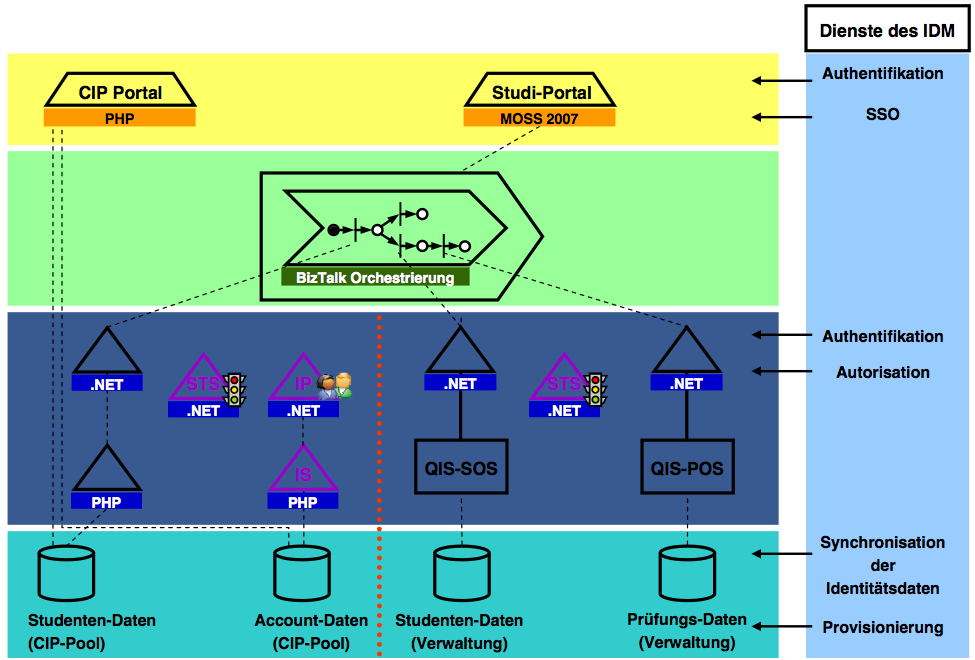
\includegraphics[width=\textwidth]
	{kapitel/gruppe4_2/bilder/ubersicht_karlsruhe}
	\caption{Erreichtes im Überblick für Karlsruhe, nach Juling Best Practice Workshop 2008}
	\label{fig_ubersicht_karlsruhe}
\end{figure}

KIM ist im Ansatz eine dienstorientierte Föderation, in der die jeweiligen Fachbereiche sich an bestimmte Schnittstellen halten und selbst die Dienste in ihrer bevorzugten Art und Programmierung zur Verfügung stellen. Dabei wurde ein hoch komplexes, aber nach eigenen Angaben sehr flexibles System, im Rahmen der 5 Jahre DFG Förderung, geschaffen.\footnote{\cite{bode_informationsmanagement_2010}}

An der Universität Karlsruhe studieren (Stand 02/2014) ca. 24.500 Studenten ca. 9500 Mitarbeiter davon 346 Professoren mit Einnahmen in Mio. EUR 795 wovon Drittmittel EUR 339 Mio. betragen. Die Landesmittel sind mit EUR 212 Mio. und die Bundesmittel mit EUR 349 Mio. angegeben.\footnote{\url{https://www.kit.edu/mediathek/print_forschung/Flyer_KIT_de.pdf}} Den CIO bilden Rektorat und Vorstand.

\begin{figure}[h!]
	\centering
	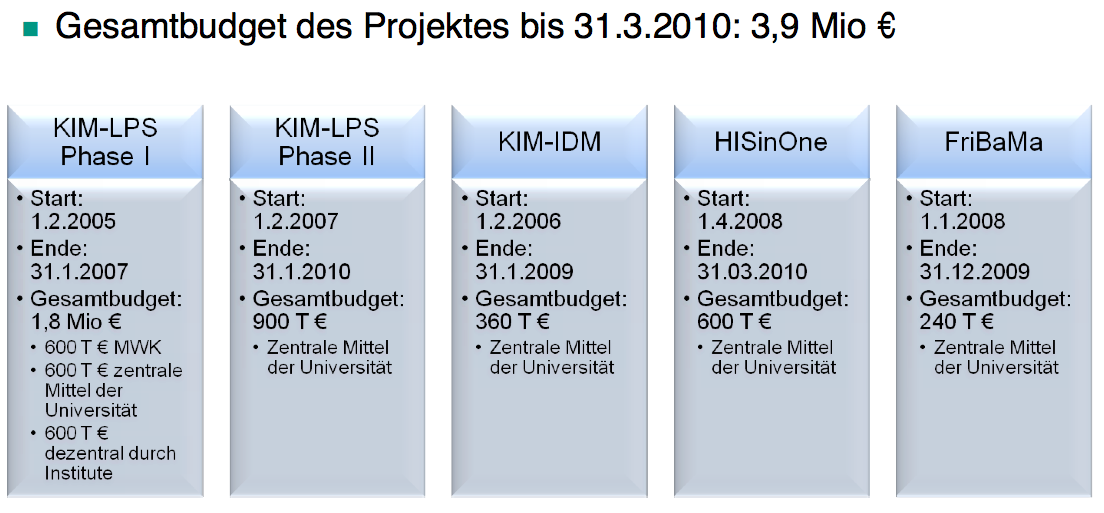
\includegraphics[width=\textwidth]
	{kapitel/gruppe4_2/bilder/uberblick_projekt_KIM}
	\caption{Erreichtes im Überblick für Karlsruhe, nach Juling Best Practice Workshop 2008}
	\label{fig_uberblick_projekt_KIM}
\end{figure}

Aus den bekannten Werten des Projektes MIRO kann nun abgeleitet werden, wieviele Personen an dem Projekt mitgewirkt haben könnten und welche Beträge für sonstige Kosten zur Verfügung standen. Diese Annahme in der Tabelle \ref{tab_minimale_investition_karlsruhe} ist rein fiktiv und dient lediglich dem Vergleich mit dem Projekt MIRO, dass den selben DFG-Förderungen gegenüber steht.

\todo[inline]{Tabelle neu formatieren}
\begin{table}[h!]
	\begin{tabularx}{\textwidth}{l|r}
		\hline
		\textbf{Kostenaufteilung Annahme KIM} & \textbf{Betrag in EUR}\\
		Gesamtvolumen über 5 Jahre & 3.900.000\\
		Personalkosten IT ca. 75\% & 2.925.000\\
		Kosten pro Projektmitarbeiter (50 möglich) & 58.500 (ca. 4.875 / Monat)\\ 
		Sonstige Kosten (unbekannt) & 975.000 (ca. 81.250 / Jahr)\\
		\hline
	\end{tabularx}
	\caption{Annahme der minimalen Investition in Karlsruhe}
	\label{tab_minimale_investition_karlsruhe}
\end{table}

Die Hochschule Emden/Leer ist mit 4.626 Studierenden eine kleine Hochschule, für die nun in Tabelle \ref{tab_kostenaufteilung_emden_MIRO} beispielhaft eine fiktive Annahme durch Teilung, aus den Werten des MIRO Projektes, gezeigt wird. Die Grundlage wäre das Minimum, dass dem MIRO Projekt durch seine DFG Förderung zukam.

\todo[inline]{Tabelle neu formatieren}
\begin{table}[h!]
	\begin{tabularx}{\textwidth}{l|r}
		\hline
		\textbf{Kostenaufteilung Annahme KIM} & \textbf{Betrag in EUR}\\
		Gesamtvolumen über 5 Jahre (fiktiv) & 169.000\\
		Personalkosten IT ca. 75\% & 126.750\\
		Kosten pro Projektmitarbeiter (2 möglich) & 63.375 (ca. 5.281 / Monat)\\ 
		Sonstige Kosten (unbekannt) & 42.250 (ca. 8.450 / Jahr)\\
		\hline
	\end{tabularx}
	\caption{Annahme der minimalen Investition in Emden; Basis gegenüber MIRO 13\%}
	\label{tab_kostenaufteilung_emden_MIRO}
\end{table}

Mit EUR 1,3 Mio. bekannten Projektmitteln, hat die Universität Münster mit ca. 37.000 Studierenden und Jahresmitteln von EUR 621 Mio. zu Emden mit EUR 36 Mio. Jahresmittel und ca. 5.000 Studierenden einen Vergleichsanteil, im Bezug auf die Anzahl der Studenten, von 13\%.

Sollte man in Emden den Wert des Projektes etwas besser bewerten, kann man die Grundlage für das Minimum aus dem KIM Projekt durch seine DFG Förderung plus die Zuwendungen durch Zentral Mittel der Universität kalkulieren. Damit würde dem Projekt ein finanzielles Volumen wie in Tabelle \ref{tab_kostenaufteilung_emden_KIM} zustehen.

\todo[inline]{Tabelle neu formatieren}
\begin{table}[h!]
	\begin{tabularx}{\textwidth}{l|X}
		\hline
		\textbf{Kostenaufteilung Annahme KIM} & \textbf{Betrag in EUR}\\
		Gesamtvolumen über 5 Jahre (fiktiv) & 169.000\\
		Personalkosten IT ca. 75\% & 126.750\\
		Kosten pro Projektmitarbeiter (2 möglich) & 63.375 (ca. 5.281 / Monat)\\ 
		Sonstige Kosten (unbekannt) & 42.250 (ca. 8.450 / Jahr)\\
		\hline
	\end{tabularx}
	\caption{Annahme der minimalen Investition in Emden; Basis gegenüber KIM 20\%}
	\label{tab_kostenaufteilung_emden_KIM}
\end{table}

Bei einem anzunehmenden Mittelwert von ca. EUR 4.916 für Personal in Emden, würde etwas mehr Geld für die Position Personal benötigt oder es wird eine weniger oder eine halbe Stelle angesetzt. Mit EUR 3,9 Mio. hat die Universität Karlsruhe mit ca. 25.000 Studierenden und Jahresmittel von EUR 795 Mio.  zu Emden mit EUR 36 Mio. Jahresmittel und ca. 5.000 Studierenden einen Vergleichsanteil, im Bezug auf die Anzahl der Studenten, von 20\%.